
% ---------------------- Эксперимент 1 ----------------------
\section{Игра на реакцию (вариант 13)}
\subsection*{Условие по варианту}
\begin{itemize}
	\item Начальное состояние светодиодов: \textbf{включены} (знак «+» в таблице).
	\item Направление циклического движения: \textbf{справа} (светодиоды загораются последовательно справа налево).
	\item Количество светодиодов: \textbf{6}.
\end{itemize}
При нажатии на кнопку из бегущей последовательности выбирается только один светодиод (фиксация случайного момента). Схема собрана без использования Arduino и программирования.

\begin{figure}[H]
	\centering
	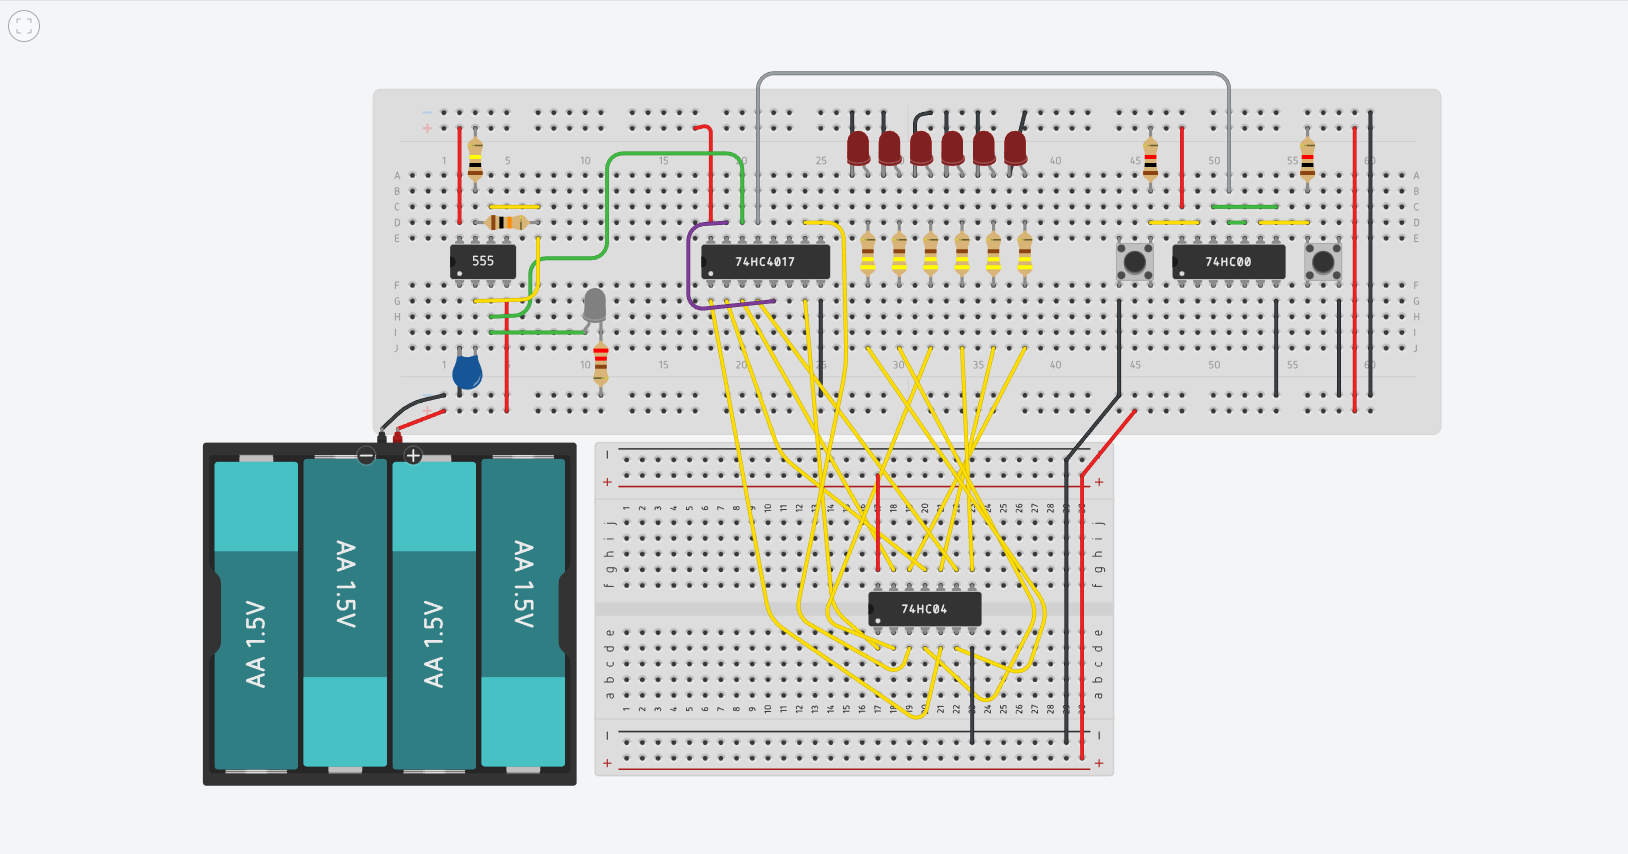
\includegraphics[width=17cm]{z1/0.png}
	\caption{Схема сборки}
\end{figure}

\begin{figure}[H]
	\centering
	
\includegraphics[width=17cm]{z1/1.png}
	\caption{Принципиальная схема ч.1}
\end{figure}

\begin{figure}[H]
	\centering
	
\includegraphics[width=17cm]{z1/2.png}
	\caption{Принципиальная схема ч.2}
\end{figure}

\subsection*{Ссылка на рабочий проект}
\url{https://www.tinkercad.com/things/2wlgeDbk03s-l3z1?sharecode=DB_PzyGiwilQSUGEBgWmMIwVAxR5XvV4WwWLfSuhy9M}

\noindent
В проекте реализован бегущий огонь на 6 светодиодах с управлением от кнопки (выбор одного светодиода). Используются сдвиговые регистры и таймер 555 для генерации тактов.

% ---------------------- Эксперимент 2 ----------------------
\newpage
\section{Декодер (вариант 13)}
\subsection*{Условие по варианту}
\begin{itemize}
	\item Начальное число задаётся переключателем в \textbf{двоичном} коде (4 бита).
	\item Преобразование: двоичный код $\rightarrow$ код Грея.
	\item Смещение результата: $+13$ (т.е. к полученному коду Грея прибавляется число 13, затем результат выводится на светодиоды в двоичной форме).
\end{itemize}
Запрещено использовать микросхему сумматора. Разрешены логические элементы 74HC04, 74HC86, 74HC32, 74HC08.

\begin{figure}[H]
	\centering
	
\includegraphics[width=17cm]{z2/0.png}
	\caption{Схема сборки}
\end{figure}

\begin{figure}[H]
	\centering
	
\includegraphics[width=17cm]{z2/1.png}
	\caption{Принципиальная схема ч.1}
\end{figure}

\begin{figure}[H]
	\centering
	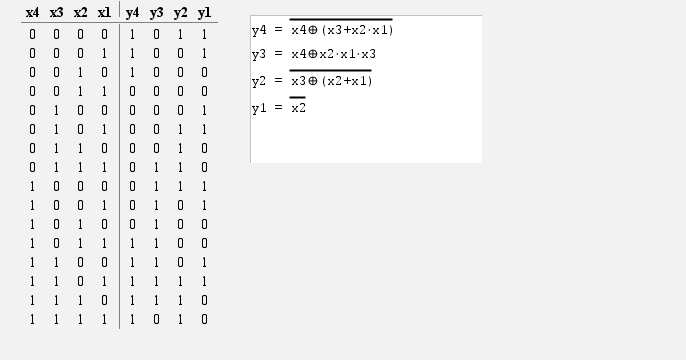
\includegraphics[width=17cm]{z2/x.png}
	\caption{Таблица истинности и формулы}
\end{figure}

\subsection*{Ссылка на рабочий проект}
\url{https://www.tinkercad.com/things/936sfZ1L713-l3z2?sharecode=9oa_ye58lNOYYU49e2HYsgFV54-JXeO-KtlbIti9U-k}

% ---------------------- Эксперимент 3 ----------------------
\newpage
\section{Декодер+ (вариант 13)}
\subsection*{Условие по варианту}
\begin{itemize}
	\item Начальное число – 3-битный \textbf{двоичный} код. 
	\item Выходное число – 7-битный код «Термометр» (термометрический код, где количество единиц равно значению числа).
	\item Используемые микросхемы: \textbf{74HC32} (OR) и \textbf{74HC08} (AND).
\end{itemize}
Преобразование реализуется комбинационной логикой без программирования.

\begin{figure}[H]
	\centering
	
\includegraphics[width=17cm]{z3/0.png}
	\caption{Схема сборки}
\end{figure}

\begin{figure}[H]
	\centering
	
\includegraphics[width=17cm]{z3/1.png}
	\caption{Принципиальная схема ч.1}
\end{figure}

\begin{figure}[H]
	\centering
	
\includegraphics[width=17cm]{z3/2.png}
	\caption{Принципиальная схема ч.2}
\end{figure}

\begin{figure}[H]
	\centering
	
\includegraphics[width=17cm]{z3/x.png}
	\caption{Таблица истинности и формулы}
\end{figure}


\subsection*{Ссылка на рабочий проект}
\url{https://www.tinkercad.com/things/2c9JElOjNOU-l3z3?sharecode=Z-9qWIKNeuXlnMeC_AkCUUgPS2dOu5rN7X838zCk9iU}
% ---------------------- Эксперимент 4 ----------------------
\newpage
\section{Секундомер (вариант 13)}
\subsection*{Условие по варианту}
\begin{itemize}
	\item Последовательность отображаемых чисел: \textbf{нечётные} от 0 до 99 (1, 3, 5, …, 99).
	\item Сброс (счёт начинается сначала) происходит при достижении числа \textbf{83}.
\end{itemize}
Схема реализована на счётчиках и логических элементах, без Arduino.

\begin{figure}[H]
	\centering
	
\includegraphics[width=17cm]{z4/0.png}
	\caption{Схема сборки}
\end{figure}

\begin{figure}[H]
	\centering
	
\includegraphics[width=17cm]{z4/1.png}
	\caption{Принципиальная схема ч.1}
\end{figure}

\begin{figure}[H]
	\centering
	
\includegraphics[width=17cm]{z4/2.png}
	\caption{Принципиальная схема ч.2}
\end{figure}

\begin{figure}[H]
	\centering
	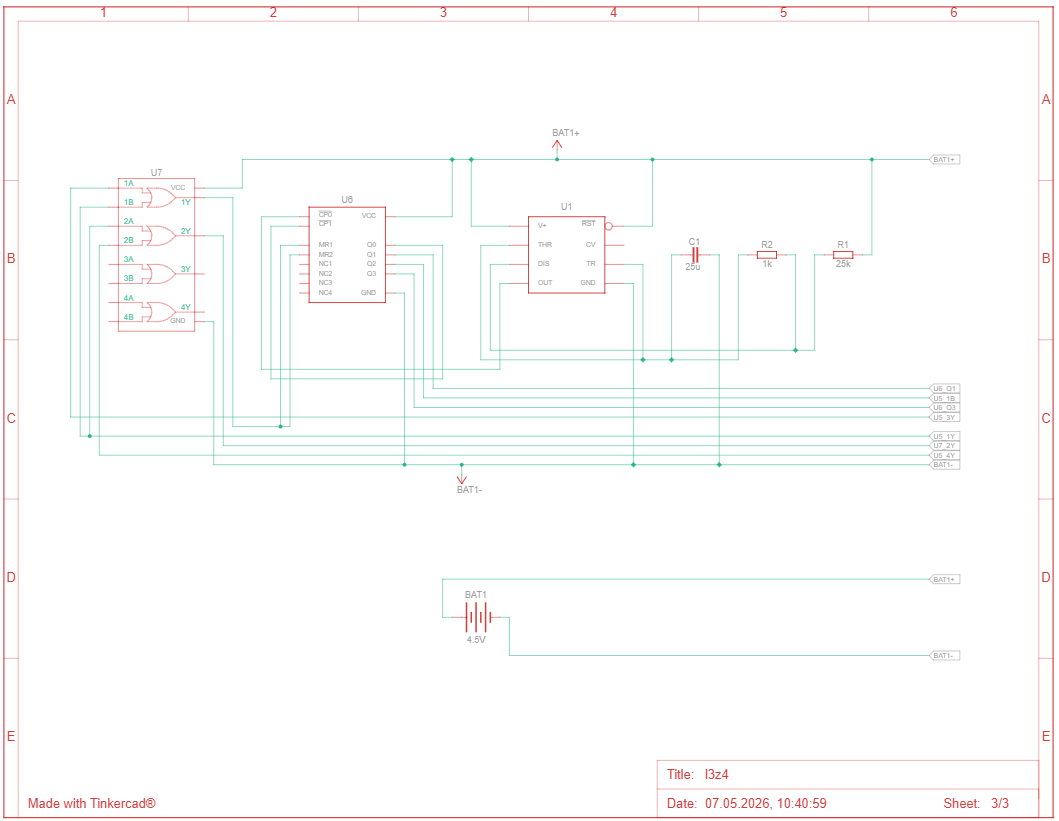
\includegraphics[width=17cm]{z4/3.png}
	\caption{Принципиальная схема ч.3}
\end{figure}

\subsection*{Ссылка на рабочий проект}
\url{https://www.tinkercad.com/things/0fD9iNtFTNa-l3z4?sharecode=Hk4DchRscwcwfyFa3AATBzpfUVvMH1XbEppzD-mhOFY}

% ---------------------- Эксперимент 5 ----------------------
\newpage
\section{Секундомер+ (вариант 13)}
\subsection*{Условие по варианту}
\begin{itemize}
	\item Счёт с шагом 4: 00, 04, 08, 12, 16, …, 96, затем сброс и повтор.
	\item Допустимые числа только кратные 4 (00, 04, 08, …, 96).
\end{itemize}

\begin{figure}[H]
	\centering
	
\includegraphics[width=17cm]{z5/0.png}
	\caption{Схема сборки}
\end{figure}

\begin{figure}[H]
	\centering
	
\includegraphics[width=17cm]{z5/1.png}
	\caption{Принципиальная схема ч.1}
\end{figure}

\begin{figure}[H]
	\centering
	
\includegraphics[width=17cm]{z5/2.png}
	\caption{Принципиальная схема ч.2}
\end{figure}

\subsection*{Ссылка на рабочий проект}
\url{https://www.tinkercad.com/things/0jzAl01p35U-l3z5?sharecode=YYv1C4eRDJ45LtvSSXwr_agcncXQ933AuRm0YgQSqCY}


% \section*{Задание 1: Кнопочные ковбои}
% \begin{verbatim}
% 					Начальное состояние: выкл
% 					Количество игроков: 2
% 					После окончания игры: начинаем сначала
% \end{verbatim}
% \begin{figure}[H]
% 	\centering
% 	
\includegraphics[width=17cm]{z1/1.png}
% 	\caption{схема сборки}
% \end{figure}
% \newpage
% \begin{figure}[H]
% 	\centering
% 	
\includegraphics[width=17cm]{z1/2.png}
% 	\caption{принципиальная схема}
% \end{figure}
% % \newpage
% \noindent
% \textbf{Код прошивки 1:}
% \lstinputlisting{z1/code.cpp}
% \noindent
% \indent
% Код реализует игровую логику для двух участников.
% После случайной паузы подается звуковой сигнал,
% и игроки соревнуются в скорости нажатия на свои кнопки.
% Тот, кто нажал первым, получает очко и включает один из своих светодиодов.
% При достижении трех очков светодиоды победителя мигают,
% затем все очки обнуляются и игра продолжается.
% Зуммер используется для подачи сигналов старта и победы. \\
% \newline
% \section*{Задание 2: Вывод текста}
% \indent
% Используя дисплей МЭЛТ вывести свое имя и фамилию в верхнем регистре на русском языке на
% LCD дисплей. \\
% \newline
% \noindent
% \textbf{Код прошивки 2:}
% \lstinputlisting{z2.cpp}
% \noindent
% \indent
% Данный код управляет символьным ЖК-дисплеем.
% В начале выполняется настройка интерфейса и инициализация дисплея с размерностью 16x2 символов.
% После очистки экрана в первой строке выводится Имя.
% Во второй строке отображается Фамилия.
% Основной цикл программы остается пустым,
% поэтому дисплей статически показывает заданное сообщение без изменений.
% \section*{Задание 3: Тестер батареек}
% \begin{verbatim}
% 					ЖК экран: I2C
% 					Движение строки: Слева-направо
% 					По кнопке: Смена направления
% 					На второй строке отображать: Время работы программы
% \end{verbatim}
% \begin{figure}[H]
% 	\centering
% 	
\includegraphics[width=17cm]{z3/1.png}
% 	\caption{схема сборки}
% \end{figure}
% % \newpage
% \begin{figure}[H]
% 	\centering
% 	
\includegraphics[width=17cm]{z3/2.png}
% 	\caption{принципиальная схема}
% \end{figure}
% \newpage
% \noindent
% \textbf{Код прошивки 3:}
% \lstinputlisting{z3/code.cpp}
% \noindent
% \indent
% Данный код отображает на дисплее бегущую строку с напряжением и время работы устройства.
% Он считывает аналоговый сигнал с батареи,
% корректирует его с учётом падения напряжения на диоде и выводит
% полученное значение на первой строке в виде бегущей строки.
% Направление бегущей сторки меняется при нажатии кнопки.
% \newpage
% \section*{Задание 4: Секундомер}
% \begin{verbatim}
% 					Последовательность: числа Фибоначчи (A000045)
% 					Сборка (общ.): катод
% \end{verbatim}
% \begin{figure}[H]
% 	\centering
% 	
\includegraphics[width=17cm]{z4/1.png}
% 	\caption{схема сборки}
% \end{figure}
% \newpage
% \begin{figure}[H]
% 	\centering
% 	
\includegraphics[width=17cm]{z4/2.png}
% 	\caption{принципиальная схема}
% \end{figure}
% \newpage
% \noindent
% \textbf{Код прошивки 4:}
% \lstinputlisting[language=Python]{z4/code.cpp}
% \noindent
% \indent
% Код для Arduino вычисляет числа Фибоначчи до 99, сохраняя их в массив. Затем он циклически отображает каждое число.
% \newpage
% \section*{Задание 5: Секундомер на 4511}
% \begin{verbatim}
% 					Последовательность: Полупростые числа (A001358)
% 					Сборка (общ.): анод
% \end{verbatim}
% \begin{figure}[H]
% 	\centering
% 	
\includegraphics[width=17cm]{z5/1.png}
% 	\caption{схема сборки}
% \end{figure}
% \newpage
% \begin{figure}[H]
% 	\centering
% 	
\includegraphics[width=17cm]{z5/2.png}
% 	\caption{принципиальная схема ч.1}
% \end{figure}
% % \newpage
% \begin{figure}[H]
% 	\centering
% 	
\includegraphics[width=17cm]{z5/3.png}
% 	\caption{принципиальная схема ч.2}
% \end{figure}
% \newpage
% \begin{figure}[H]
% 	\centering
% 	
\includegraphics[width=17cm]{z5/4.png}
% 	\caption{принципиальная схема ч.3}
% \end{figure}
% % \newpage
% \begin{figure}[H]
% 	\centering
% 	
\includegraphics[width=17cm]{z5/5.png}
% 	\caption{принципиальная схема ч.4}
% \end{figure}
% \newpage
% \textbf{Код прошивки 5:}
% \lstinputlisting[language=Python]{z5/code.cpp}
% \noindent
% \indent
% Данный код управляет выводом двухзначных чисел на семисегментный индикатор с общим анодом. 
% Он последовательно перебирает числа от 0 до 99, отбирая только полупростые (произведение двух простых). 
% Для каждого такого числа код формирует BCD-код каждой цифры и через сдвиг подаёт его на микросхему CD4511. 
% Поскольку индикатор анодный, между CD4511 и сегментами включён инвертор 74HC04, который инвертирует уровни.
% Затем следует задержка, после чего перебор продолжается.
% \newpage
% \section*{Задание 6: Сборка счетчика нажатий на базе 595}
% \begin{verbatim}
% 					Последовательность: Счастливые числа (A000959)
% 					Сборка (общ.): секундомер
% \end{verbatim}
% \begin{figure}[H]
% 	\centering
% 	
\includegraphics[width=17cm]{z5/1.png}
% 	\caption{схема сборки}
% \end{figure}
% \newpage
% \begin{figure}[H]
% 	\centering
% 	
\includegraphics[width=17cm]{z6/2.png}
% 	\caption{принципиальная схема ч.1}
% \end{figure}
% % \newpage
% \begin{figure}[H]
% 	\centering
% 	
\includegraphics[width=17cm]{z6/3.png}
% 	\caption{принципиальная схема ч.2}
% \end{figure}
% \newpage
% \textbf{Код прошивки 6:}
% \lstinputlisting[language=Python]{z6/code.cpp}
% \newpage
% \noindent
% \indent
% Данный код управляет сдвиговыми регистрами 74HC595 для вывода на двухразрядный семисегментный индикатор с общим катодом.
% В начале выполняется инициализация пинов и формирование массива по алгоритму, напоминающему «счастливые числа»:
% из последовательности 0..99 удаляются элементы, номера которых кратны текущему ненулевому значению.
% В результате остаются только определённые числа.
% Основной цикл поочерёдно отображает двузначные числа из этого отфильтрованного списка.
% Для каждого числа формируется 16-битная маска (по байту на разряд),
% которая побитно сдвигается в регистр. После передачи всех битов данные фиксируются на выходах,
% и индикатор показывает текущее число в течение 1.5 секунд.
% Затем выбирается следующее подходящее число, и процесс повторяется. \\
% \newline

% \noindent
% \textbf{Ссылки на рабочие проекты:}
% \begin{enumerate}
% 	\item Кнопочные ковбои \href{https://www.tinkercad.com/things/fRYbcPVnXsc-p2z1?sharecode=ate8HW4nB-33PNui2slqs1_fwZmyqGUiU90PzT0SCSc}{(тинкеркад)}
% 	\item Вывод текста (сборка в живую)
% 	\item Тестер батареек \href{https://www.tinkercad.com/things/59G80bUWjiw-p2z3?sharecode=7pNuAb2y5_4BliYQ4GSQSyR5lI0uoTwBuljGs1v808w}{(тинкеркад)}
% 	\item Секундомер \href{https://www.tinkercad.com/things/ckRnPBFQeNo-p2z4?sharecode=6DJ-QDE7lFqlMGE6p0FtlmDj3fhivjqegiAksTsGnoM}{(тинкеркад)}
% 	\item Секундомер на 4511 \href{https://www.tinkercad.com/things/2kjGxK0594n-p2z5?sharecode=XUadcWefD3XcFySOLOHOt79jrYyJvvpEVuWAdU66WuA}{(тинкеркад)}
% 	\item Сборка счетчика нажатий на базе 595 \href{https://www.tinkercad.com/things/1gCfMsY0VKK-p2z6?sharecode=uf8FhYgYr-Il7vByz92F_BKAfCqUqiK4jTCHH8xt6xY}{(тинкеркад)}
% \end{enumerate} 
